\documentclass[slovene,11pt,a4paper]{article}
\usepackage[margin=1.8cm,bottom=3cm,foot=1.5cm]{geometry}
\usepackage{amsmath}
\usepackage{booktabs}
\usepackage{float}
\usepackage{graphicx}
\usepackage{gensymb}
\usepackage{geometry}
\usepackage{changepage}
\usepackage{subcaption}
\usepackage{multirow}
\usepackage{blindtext}
\usepackage{hyperref}
\usepackage[version=4]{mhchem}
\usepackage[slovene]{babel}
\pagenumbering{gobble}
\renewcommand{\contentsname}{\centering Contents}

\begin{document}

\title{9. naloga - Stohastični populacijski modeli}
\author{Tadej Lozej 28201055}
\maketitle
\begin{center}
Modelska analiza 1 \\
\bigskip
Predavatelj: prof. dr. Simon Širca \\
Asistent: doc. dr. Miha Mihovilovič
\end{center}

\newpage

\tableofcontents

\newpage

\section{Uvod}

\pagenumbering{arabic}

Populacijske modele smo raziskali že v četrti nalogi modelske analize. Podobne primere bomo obravnavali še enkrat, a tokrat stohastično. Diskretizirali bomo vrednosti populacije ter na podlagi Poissonove porazdelitve sprejemali odločitve.

\section{Statistika časov izumrtja}

Imamo preprost eksponentno izumirajoči model populacije

\begin{equation}
\dot{N} = -\beta N; \quad N(0) = N_0,
\end{equation}
kjer je $\beta = 1.0/\text{enota časa}$ koeficient hitrosti izumiranja ter $N$ število osebkov v populaciji. To diferencialno enačbo lahko rešimo eksaktno in preprosto dovolimo, da populacija zvezno upada, ker ni nujno res, saj moramo načeloma ob nekem času imeti ne celo število osebkov. Model zato obravnavamo lahko tudi stohastično. Diskretiziramo čas in ob vsakem časovnem koraku po Poissonovi porazdelitvi žrebamo koliko osebkov $\Delta N$ umre. Tako ob vsakem časovnem koraku $\Delta t$ populaciji prištejemo (oz. odštejemo)

\begin{equation}
\Delta N = N - \wp (\beta N \Delta t).
\end{equation}
Na sliki 1 so prikazani poteki izumiranja za različne velikosti populacije ter zvezen model. Vidimo, da večja kot je populacija bolj se približamo zveznemu modelu.

\begin{figure}[h!]
\centering
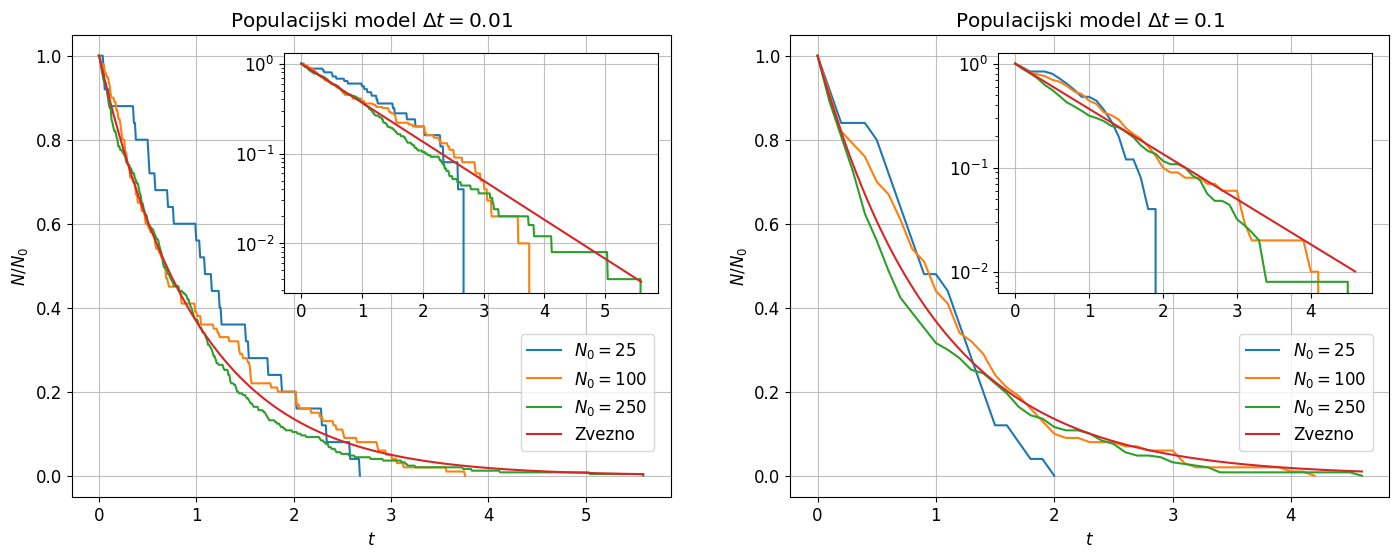
\includegraphics[width=\linewidth]{slika1.png}
\caption{Potek izumiranja za različne velikosti populacije. Vidimo, da večja kot je populacija bolj se približamo zveznemu modelu.}
\end{figure}

Seveda pa zaradi naključnega žrebanja umrlih ob vsakem času $\Delta t$ dobimo različne poteke izumrtja. Zanimala nas bo statistika časa izumrtja $t_{death}$ v odvisnosti od velikosti časovnega koraka $\Delta t$ ter velikosti populacije $N_0$. Na sliki 2 je prikazanih več potekov izumrtja za majhno $N_0=25$ ter veliko $N_0=250$ populacijo za dva različno velika časovna koraka. Na teh slikah vidimo kako raztrešeni so različni časovni poteki izumrtja. Predvsem na grafih z logaritemskimi skalami lahko dobimo občutek za porazdeljenost časa smrti $t_{death}$ za te štiri različne primere. Med različnimi časovnimi koraki ni videti pretežne razlike, lahko pa jasno opazimo, da je v povprečju večja populacija preživela dlje časa.

\newpage

\begin{figure}[h!]
\centering
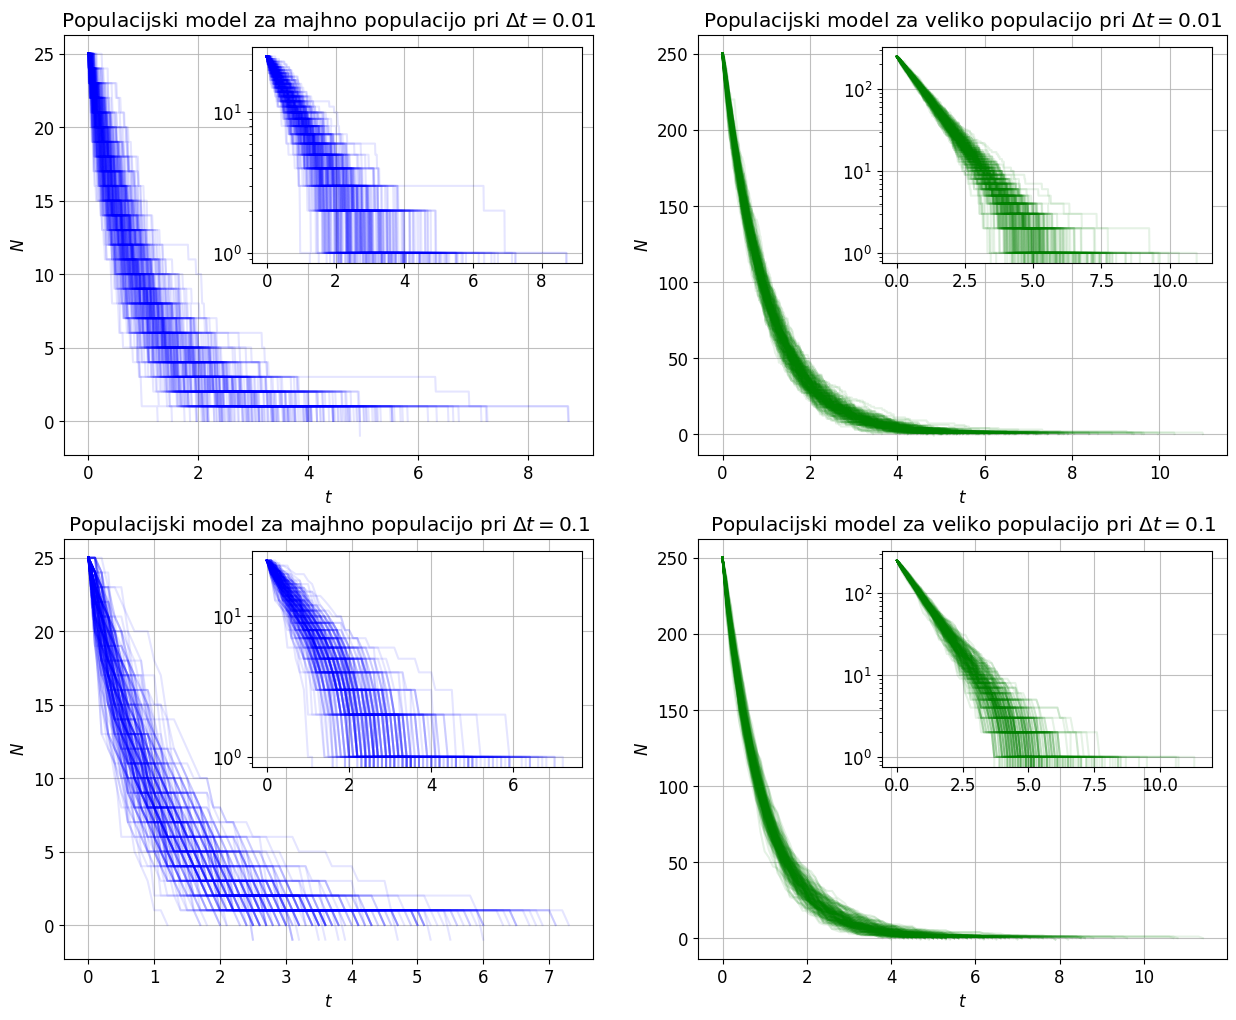
\includegraphics[width=15cm]{slika2.png}
\caption{Več potekov izumrtja za majhno $N_0=25$ ter veliko $N_0=250$ populacijo za dva različno velika časovna koraka. Vidimo raztrešenost časovnih potekov izumrtja.}
\end{figure}

Poglejmo si za začetek histogramirano porazdelitev času smrti $t_{death}$ za majhno ter veliko populacijo za nekaj različnih velikosti časovnega koraka $\Delta t$. Histogrami so prikazani na sliki 3. Predalčki po katerih sortiramo čase smrti so veliki $0.25$. Vidimo, da porazdelitev ni zares Gaussovska temveč bolj spominja na Poissonsko. Na grafih so prav podanih nekaj statističnih značilnosti porazdelitev. Sklepamo, da ima s večjim časovnim korakom porazdelitev manjše povprešje in std.

\begin{figure}[h!]
\centering
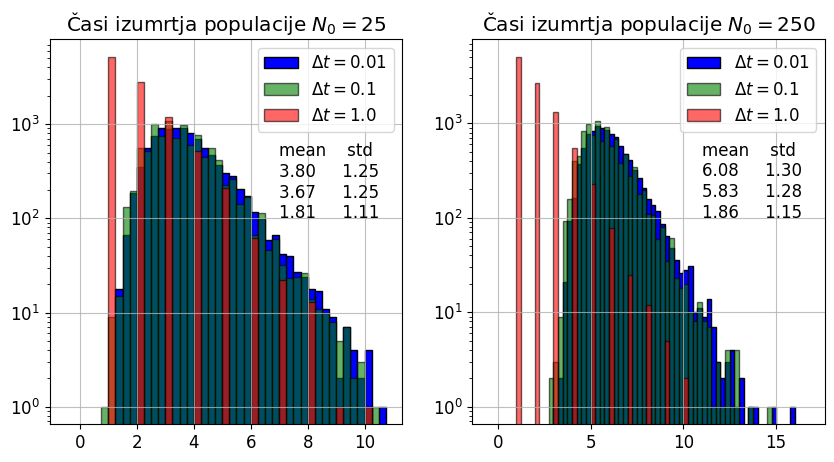
\includegraphics[width=12cm]{slika3.png}
\caption{Porazdelitev časov izumrtja populacije $t_{death}$ za majhno populacijo na levo ter veliko populacijo na desno za nekaj različnih velikosti časovnega koraka $\Delta t$.}
\end{figure}

\newpage

Na prejšnji sliki lahko vidimo statistične značilnosti le za tri primere različnih časovnih korakov. Slika 4 prikazuje tri statistične značilnosti porazdelitve časa smtri v odvisnosti od velikosti časovnega koraka $\Delta t$ za majhno in veliko populacijo. Pri povprečju, mediani in standardni deviaciji vidimo očiten trend navzdol.

\begin{figure}[h!]
\centering
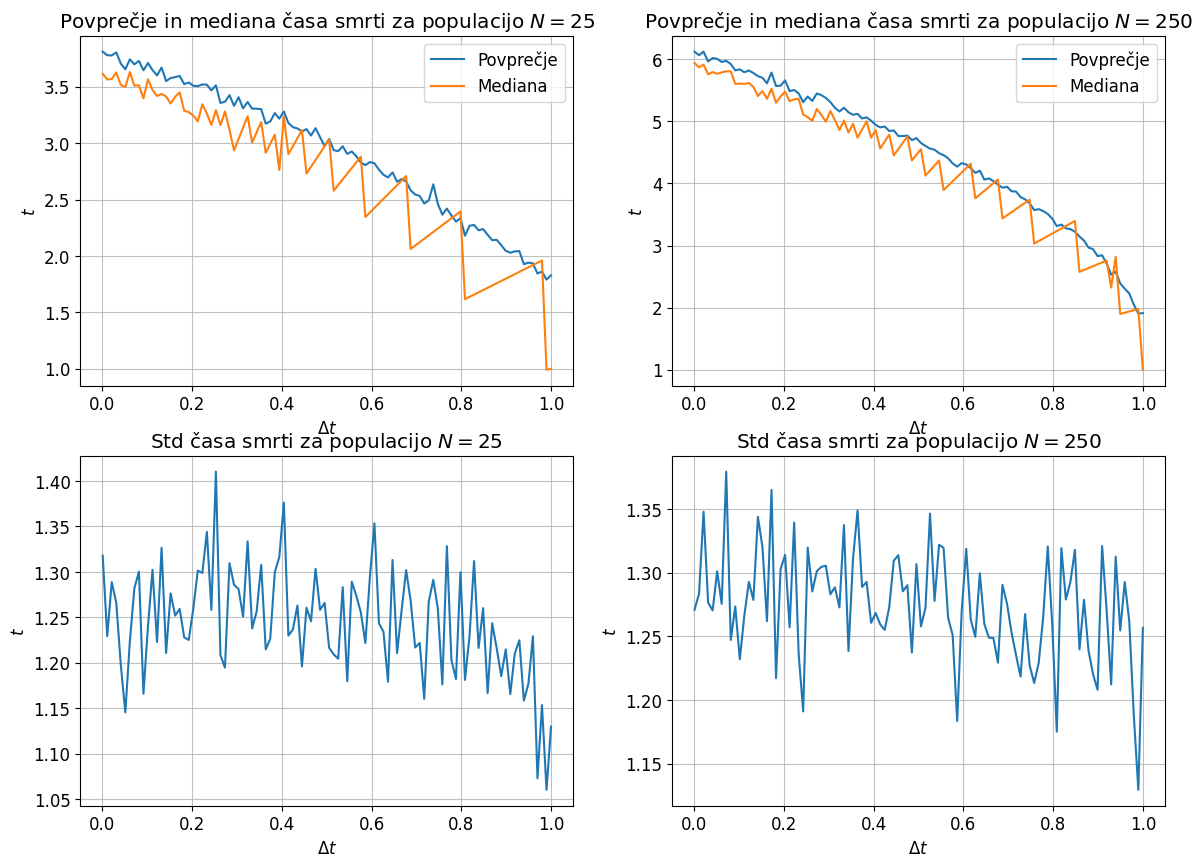
\includegraphics[width=15cm]{slika4.png}
\caption{Tri statistične značilnosti porazdelitve časa smtri v odvisnosti od velikosti časovnega koraka $\Delta t$ za majhno in veliko populacijo. Pri povprečju, mediani in standardni deviaciji vidimo očiten trend navzdol.}
\end{figure}

Podobno kot smo zdaj opazovali različne porazdelitve za različne vrednosti časovnega koraka $\Delta t$ lahko opazujemo tudi kako se med seboj razlikujejo porazdelitve z različnimi velikostmi populacije $N_0$. Na sliki 5 so prikazane tri takšne porazdelitve. Za vsako porazdelitev sem uporabil $10000$ vzorcev in predalčki so široki $0.25$ časovnih enot. Vidimo, da se povprečje porazdelitve časov smrti z večanjem populacije premika v desno, kar pomeni, da v povprečju večje populacije živijo dlje časa kot manjše. Histogrami porazdelitev so prikazani le za tri različne velikosti populacije, na sliki 6 pa lahko vidimo tri statistične lastnosti porazdelitve v odvisnosti od velikosti populacije. Očiten na prvi pogled logaritemski ali korenski trend lahko vidimo v povprečju in mediani v standardni deviaciji pa ne vidimo očitnega trenda.

\newpage

\begin{figure}[h!]
\centering
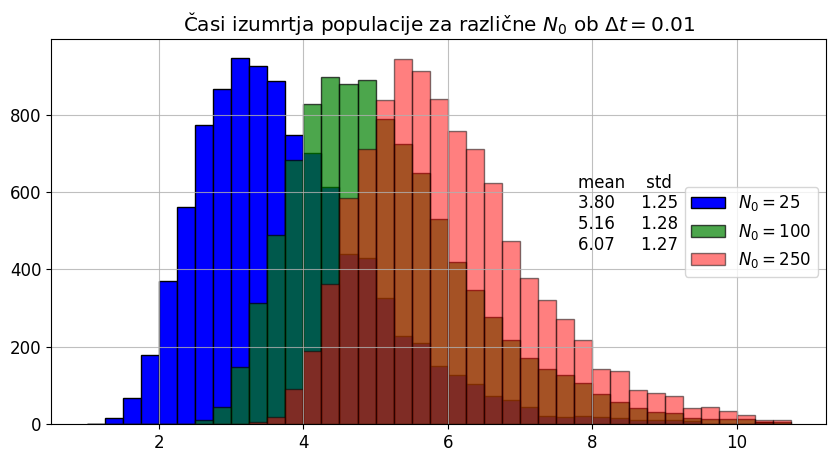
\includegraphics[width=12cm]{slika5.png}
\caption{Tri histogrami porazdelitev časa smrti za časovni korak $\Delta t = 0.01$ a različnih velikosti populacij $N_0$. Vidimo, da se z večanjem populacije porazdelitev premika v desno.}
\end{figure}

\begin{figure}[h!]
\centering
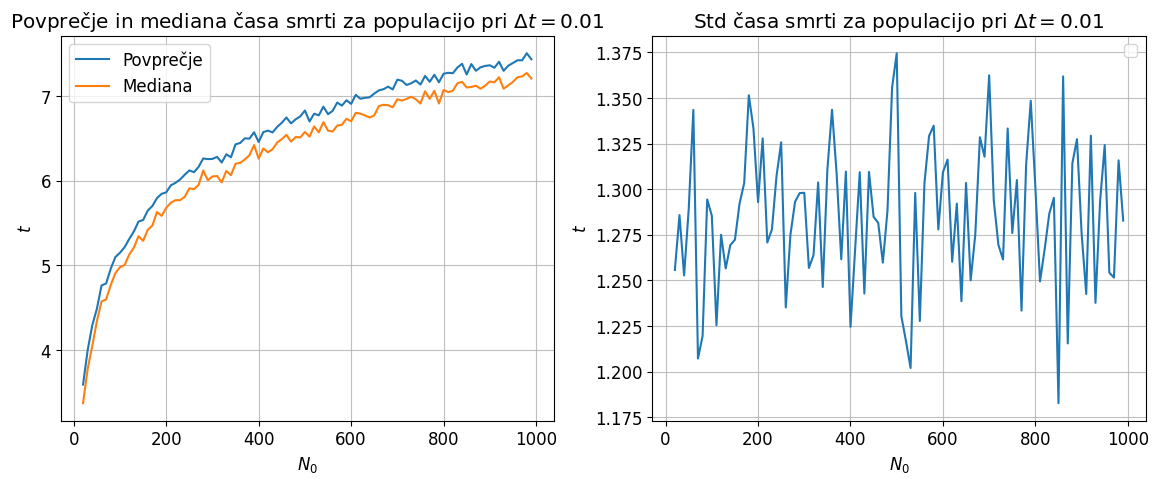
\includegraphics[width=15cm]{slika6.png}
\caption{Tri statistične lastnosti porazdelitev časa smrti v odvisnosti od velikosti populacije. Vidimo očiten naraščajoč trend za povprečje in mediano ter stagniranje standardne deviacije.}
\end{figure}

\subsection{Smrti in rojstva}

Model lahko hitro razširimo tako, da poleg smrti osebkov omogočimo tudi rojstvo le-teh. Tako ob vsakem časovnem koraku $\Delta t$ populaciji prištejemo (oz. odštejemo) spremembo populacije zaradi smrti in rojstev osebkov

\begin{equation}
\Delta N = \wp (\beta_r N \Delta t) - \wp (\beta_s N \Delta t),
\end{equation}
kjer je $\beta_r = 4\beta$ parameter, ki opisuje hitrost rojstev ter $\beta_s = 5\beta$ parameter, ki opisuje hitrost smrti.

Na sliki 7 je prikazan potek izumiranja ob dveh različno velikoh časovnih korakih za nekaj različnih velikosti populacije. Vidimo, da večja kot je populacija bolj se približamo zveznemu modelu.

\begin{figure}[h!]
\centering
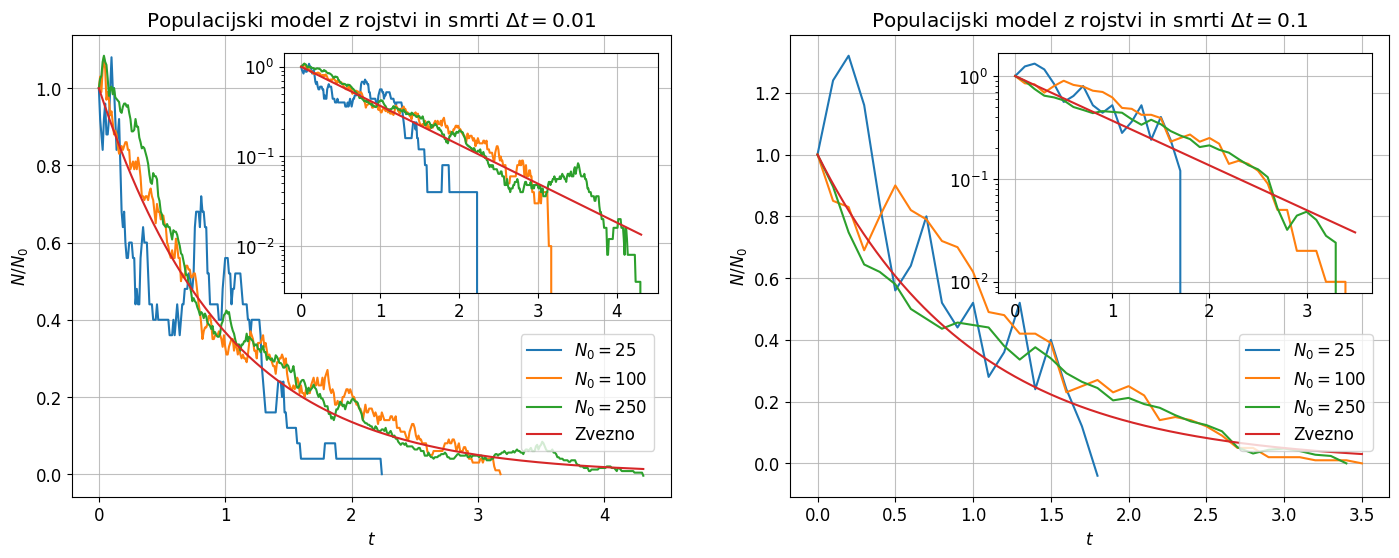
\includegraphics[width=\linewidth]{slika7.png}
\caption{Potek izumiranja za različne velikosti populacije z modelom rojstva in smrti. Vidimo, da večja kot je populacija bolj se približamo zveznemu modelu.}
\end{figure}

\newpage

Na sliki 8 si poglejmo še porazdelitve časa smrti $t_{death}$ pri fiksnem časovnem koraku $\Delta t = 0.01$ ter nekaj različnih velikosti populacije. Z večanjem populacije se kot pričakovano porezdelitve premikajo v desno. Če histograme primerjamo s prejšnjimi vidimo, da v modelu z rojstvi in smrtmi v povprečju populacija umre prej kot če imamo le smrti!

\begin{figure}[h!]
\centering
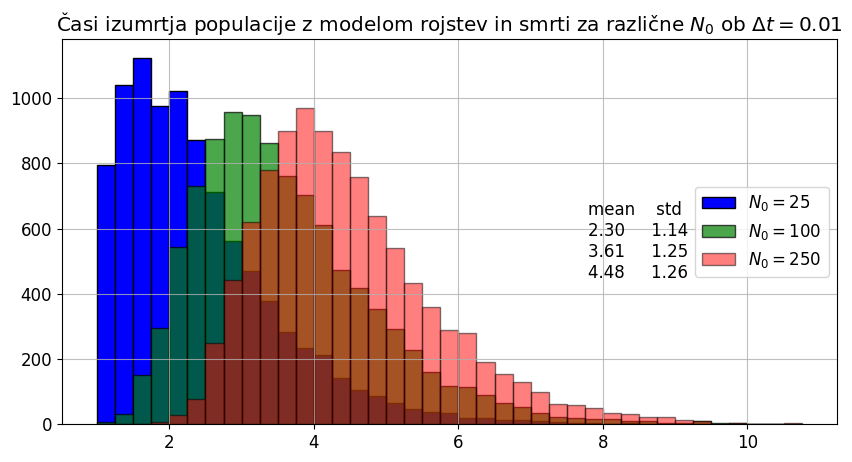
\includegraphics[width=12cm]{slika8.png}
\caption{Tri histogrami porazdelitev časa smrti za časovni korak $\Delta t = 0.01$ a različnih velikosti populacij $N_0$. Vidimo, da se z večanjem populacije porazdelitev premika v desno.}
\end{figure}

Zgoraj imamo primer le za tri različne velikosti populacije. Poglejmo si statistične lastnosti porazdelitev časa smrti $t_{death}$ v odvisnosti od velikosti populacije za model z rojstvi ter smrtmi ter jih primerjajmo z osnosnim modelom brez rojstev. Rezultati so prikazani na sliki 9. Vidimo, da sta povprečje in mediana očitno manjša pri modelu, kjer upoštevamo rojstva in smrti pri vseh velikostih populacije. Standardni odklon se pa pri modelih ne razlikuje veliko. To pomeni, da so porazdelitve približno enako široke ter imajo podobno obliko le porazdelitve časa smrti pri modelu z rojstvi in smrtmi so zamaknjene bolj v levo. V povprečju te populacije izumirajo prej.

\newpage

\begin{figure}[h!]
\centering
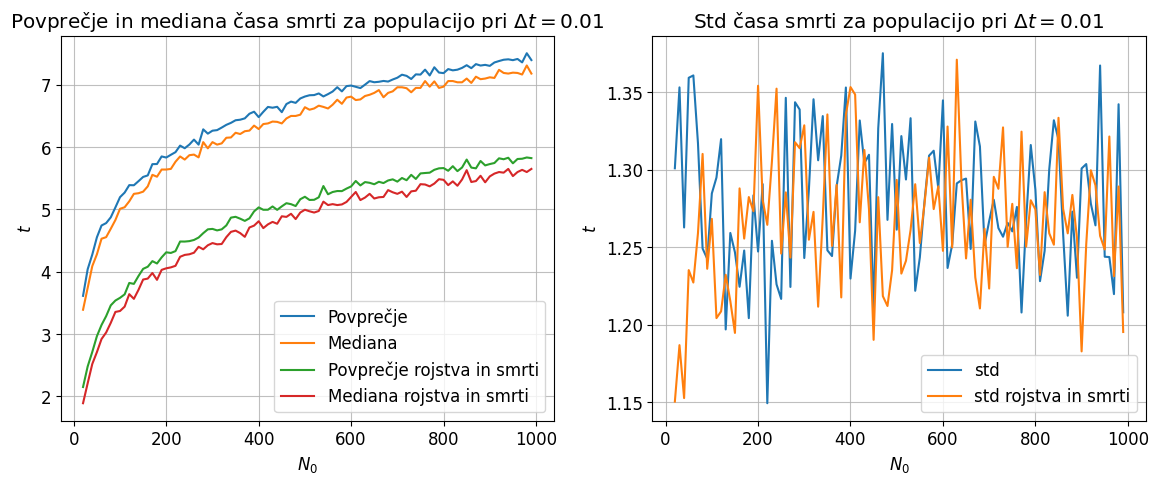
\includegraphics[width=15cm]{slika9.png}
\caption{Tri statistične lastnosti porazdelitev časa smrti v odvisnosti od velikosti populacije za model brez rojstev in model z rojstvi. Vidimo očiten naraščajoč trend za povprečje in mediano ter stagniranje standardne deviacije. Model z rojstvi ima porazdelitve očitno bolj zamaknjene v levo. To pomeni, da v povprečju te populacije prej umirajo.}
\end{figure}

\section{Matrika prehodov}

Verjetnostno porazdelitev sistema ob času $t$ opišemo z vektorjem

\begin{equation}
\vec{x}(t) = (x_1(t), x_2(t), ..., x_m(t))^T,
\end{equation}
kjer so komponente $x_j(t)$ verjetnosti, da ima sistem ob času $t$, $j$ osebkov. Začetno stanje z $N_0$ osebki bomo zapisali kot

\begin{equation}
\vec{x}(t=0) = (0, 0, ..., 1, 0, ..., 0),
\end{equation}
kjer je $1$ na mestu $N_0$. Vektorja je daljši kot začetna vrednost populacije, saj s tem omogočimo večanje populacije za $\beta_r > 0$. Prehod porazdelitve v naslednji časovni korak izračunamo kot

\begin{equation}
\vec{x}(t+\Delta t) = M\vec{x}(t),
\end{equation}
kjer matriko prehoda $M$ zapišemo kot

\begin{equation}
\begin{bmatrix}
1 & 1\beta_s \Delta t             & 0                             & 0               & ... \\
0 & 1-1(\beta_r \beta_s) \Delta t & 2\beta_s \Delta t             & 0               & ... \\
0 & 1\beta_r \Delta t             & 1-2(\beta_r \beta_s) \Delta t & 3\beta \Delta t & ... \\
... & ...                         & ...                           & ...             & ...
\end{bmatrix}
.
\end{equation}

Na sliki 10 so prikazani rezultati dobljeni z matirko prehoda za veliko populacijo. Na sliki sta poleg verjetnostne porazdelitve stanj od časa prikazana tudi prvi moment (povprečje) porazdelitve v odvisnosti od časa ter standardni odklon v odvisnosti od časa. Vidimo, da se napovedani funkciji za povprečje in std ujemata z izmerjenimi.

\newpage

\begin{figure}[h!]
\centering
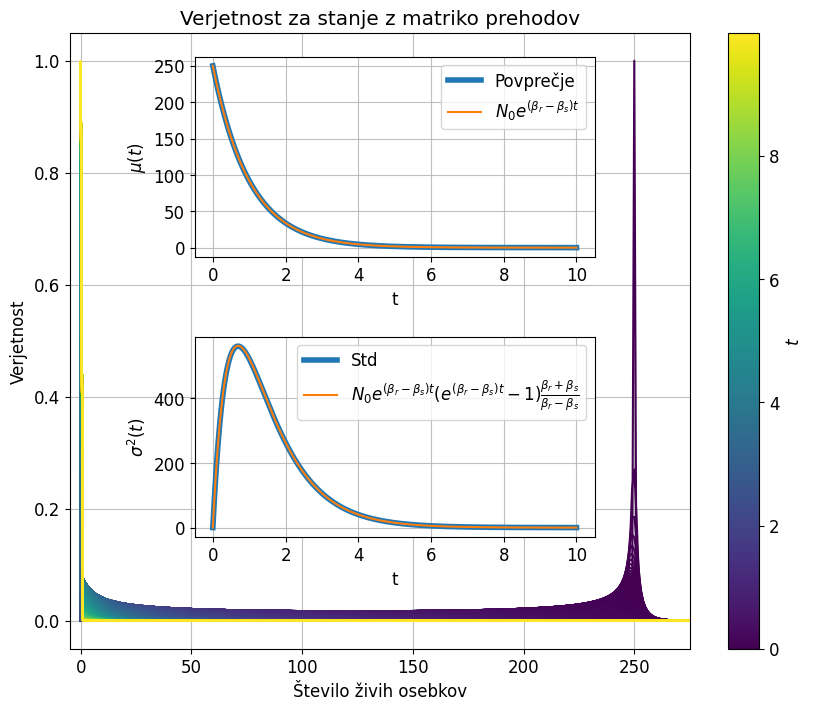
\includegraphics[width=15cm]{slika10.png}
\caption{Verjetnostna porazdelitev stanj v odvisnosti od časa pridobljena z matriko prehodov. Prikazan je tudi prvi moment (povprečje) porazdelitve v odvisnosti od časa ter standardni odklon porazdelitve.}
\end{figure}

\section{Zajci-Lisice}

S podobnim stohastičnim modelom lahko opišemo tudi problem ene od prejšnjih domačih nalog in sicer problem zajcev in lisic. S Poissonsko porazdelitvijo problem opišemo z enačbami

\begin{align}
Z_{n+1} &= Z_n + \wp(\rho_Z Z_n \Delta t) - \wp(\sigma_Z Z_n \Delta t) - \wp (\gamma Z_n L_n \Delta t) \\
L_{n+1} &= L_n + \wp(\rho_L L_n \Delta t) - \wp(\sigma_L L_n \Delta t) - \wp (\delta Z_n L_n \Delta t), \\
\end{align}
kjer so 

\[
\rho_Z = 5\alpha, \quad \sigma_Z = 4\alpha, \quad \rho_L = 4\beta, \quad \sigma_L = 5\beta, \quad \gamma = \frac{\alpha}{L_0} \quad \text{in} \quad \delta = \frac{\beta}{Z_0}.
\]
Tukaj sta $\alpha$ in $\beta$ prosta parametra ter $L_0$ ter $Z_0$ začetni vrednosti populacije lisic oz. zajcev. za vrednosti $\beta$ in $\alpha$ vzamemo kar preprosto $\beta = \alpha = 1$. Vse trajektorije oz. gledane scenarije bomo začeli v zastojni točki $(Z_0, L_0)=(200, 50)$. Na sliki 11 so prikazani trije taki scenariji v faznem prostoru lisic in zajcev. Prav tako so na spodnjih dveh grafih prikazani časovni poteki populacije lisic in populacije zajcev. Trajektorija se ustavi, ko izumrejo zajci ali lisice. V naših treh primerih v prvih dveh izumrejo lisice v tretjem pa zajci. Zanima nas statistika časa izumrtja ene izmed populacij, če začnemo v zastojni točki.

\newpage

\begin{figure}[h!]
\centering
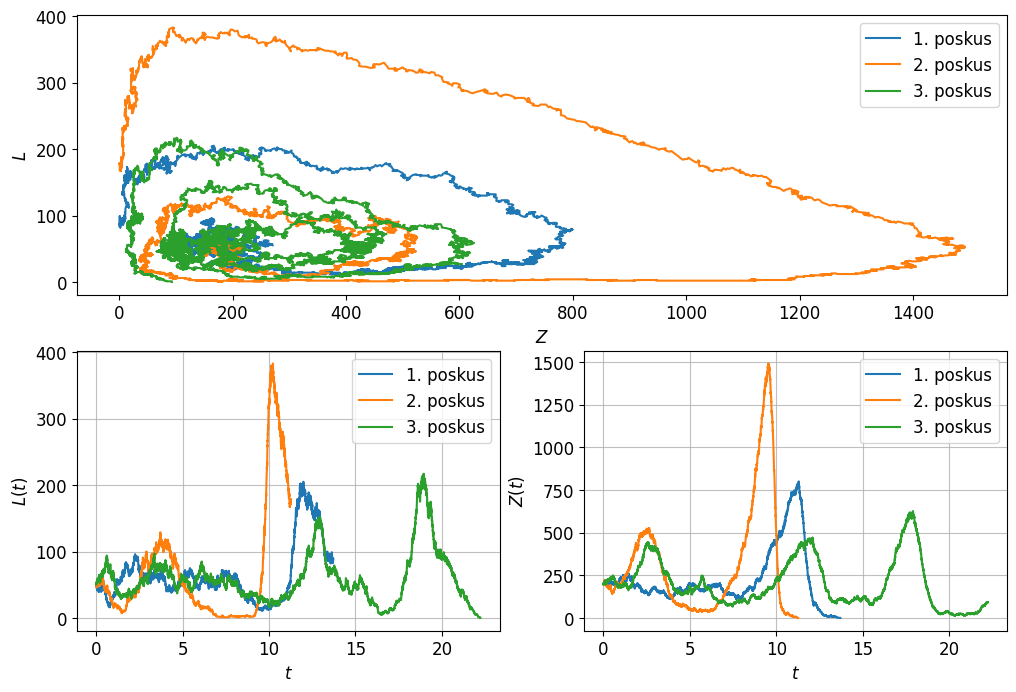
\includegraphics[width=16cm]{slika11.png}
\caption{Tri trajektorije v faznem prostoru lisic in zajcev, ki se začnejo v zastojni točki $(Z_0, L_0)=(200, 50)$.}
\end{figure}

Na sliki 12 vidimo histogram porazdelitve časov smrti sistema. Histogram vsebuje 5000 scenarijev. V teh 5000 scenarijih so lisice izumrle večkrat, in sicer 77,3\% scenarijev.

\begin{figure}[h!]
\centering
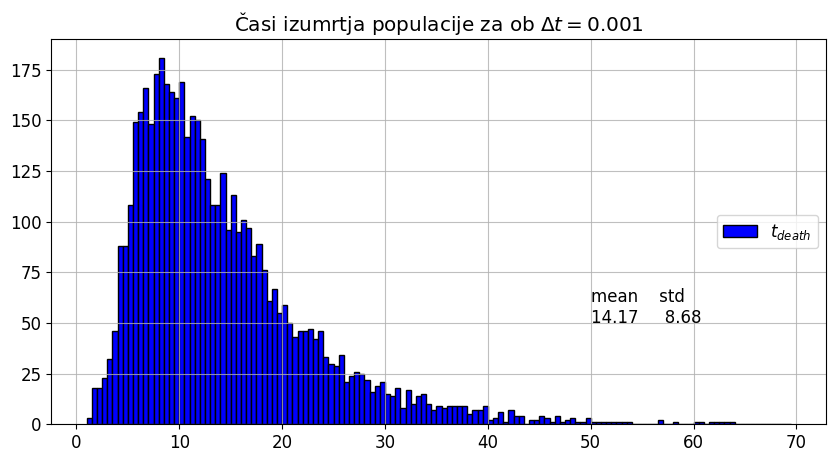
\includegraphics[width=16cm]{slika12.png}
\caption{Histogram porazdelitve časov izumrtja scenarijev, ki se začnejo v zastojni točki $(Z_0, L_0)=(200, 50)$.}
\end{figure}

\section{Epidemija}

Prav tako lahko stohastično obravnavamo model epidemije, ki smo ga zvezno obravnavali v četrti nalogi pri populacijskih modelih. V takšni obravnavi lahko brez reševanja zakasnelih diferencialnih enačb v sistemu upoštevamo to, da imuni čez nekaj časa postanejo spet dovzetni. Stohastični model zapišemo kot

\begin{align}
D_{n+1} &= D_n - a + b \\
B_{n+1} &= B_n + a - c \\
I_{n+1} &= I_n + c - b,
\end{align}
kjer so

\[
a = \wp (\alpha D_n B_{n-n_i} \Delta t), \quad
b = \wp (\gamma I_{n-n_d} \Delta t), \quad \text{in} \quad
c = \wp (\beta B_n \Delta t)
\]
Poissonsko žrebana naključna števila. Pomembno je, da v vsakem koraku števila $a$, $b$ in $c$ žrebamo le enkrat ter jih nato upoštevamo v enačbah (11)-(13), saj se tako število celotne populacije ohranja! V teh Poissonsko porazdeljenih številih imamo tudi parametre $\alpha$, $\beta$ in $\gamma$, ki upoštevajo nalezljivost bolezni (večji kot je $\alpha$ bolj je nalezljiva bolezen), hitrost prebolevanja (večji kot je $\beta$ hitreje osebek preboli bolezen) ter hitrost izgube imunosti (večji kot je $\gamma$ hitreje osebek izgubi imunost). Parametra $n_i$ in $n_d$ pa narekujeta trajanje inkubacijske dobe ter trajanje imunosti.

Na sliki 13 vidimo primer poteka epidemija za parametre zapisane na sliki. Vidimo, da je v primeru drugi val epidemije hujši kot prvi. To povzroči rast števila imunih in nato padec bolnih na $0$ in konec epidemije.

\begin{figure}[h!]
\centering
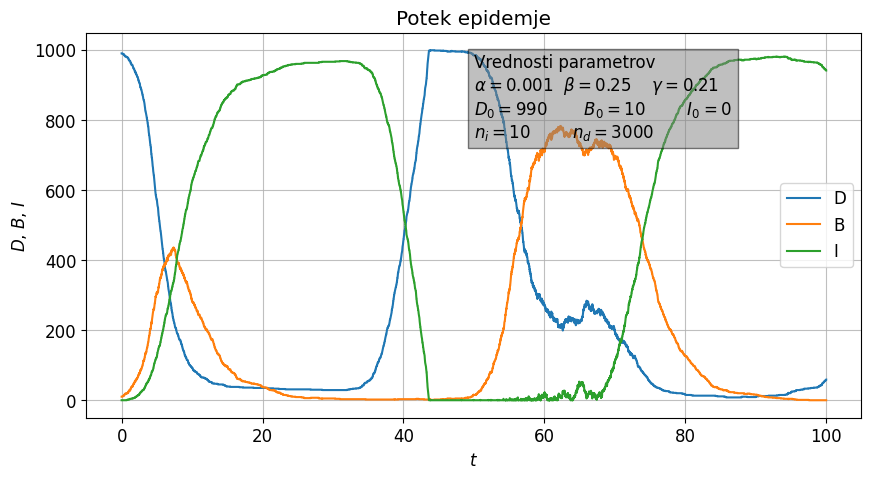
\includegraphics[width=16cm]{slika13.png}
\caption{Potek epidemije za vrednosi parametre zapisane na sliki.}
\end{figure}

Za vsak scenarij epidemije začnemo z enim procentom bolanih in 99\% dovzetnih populacije. Tako začnemo spreminjati velikost populacije $N$ ter parameter $\gamma$. Druge parametre ohranimo pri enaki vrednosti kot na sliki 13. Za vsako kombinacijo parametrov simuliramo 200 scenarijev (kar ni veliko) in si zabeležimo povprečni čas konca epidemije ter standardni odklon porazdelitve. Rezultati so prikazani na sliki 14. Zanimivo, da za izbrane parametre ne vidimo nobenega izrazitega trenda.

\begin{figure}[h!]
\centering
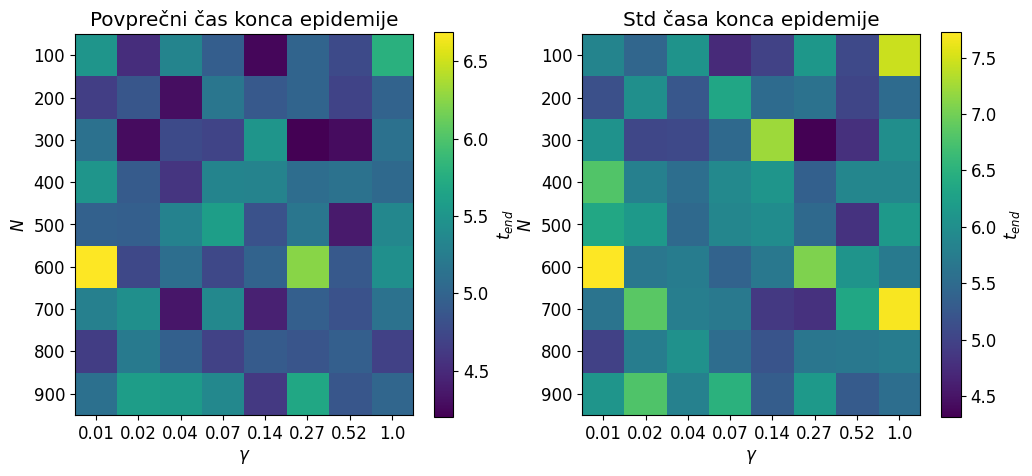
\includegraphics[width=16cm]{slika14.png}
\caption{Povprečen čas in standardno odstopanje konca epidemije v odvisnosti od velikosti populacije ter parametru $\gamma$.}
\end{figure}

\section{Zaključek}

Stohastično smo obravnavali različne populacijske modele. Model eksponentnega izumrtja, model zajcev in lisic ter model epidemije. Predvsem nas je zanimala statistika nekih karakterističnih časov.

\end{document}